\documentclass[paper=A4,pagesize=auto,11pt]{scrartcl}
%
\usepackage[margin=2.2cm]{geometry}
\usepackage[utf8]{inputenc}
\usepackage[english]{babel}
\usepackage{booktabs}
\usepackage{hyperref}
\usepackage{graphicx}
\usepackage{amsmath,amssymb}
\usepackage{latexsym}
\usepackage{eurosym}
\usepackage{units}
%
\providecommand{\gquote}[1]{`#1'}  
\newcommand{\refkl}[1]{(\ref{#1})}
\newcommand{\D}{\text{d}}
\newcommand{\sub}[1]{_\text{#1}}
\newcommand{\assupIDM}{a'^{\ \text{IDM}}} % latex bug \sup{..} geht auch
                                      % mit renewcommand nicht
\renewcommand{\sup}[1]{^{\text{#1}}}
\providecommand{\abl}[2] {\frac{\D #1}{\D #2}}
%% \newcommand{\ake}[1]{[ARNE:]\textit{#1}}
\providecommand{\bi}{\begin{itemize}}
\providecommand{\ei}{\end{itemize}}

%%%%%%%%%%%%%%%%%%%%%%
\title{Interactive Traffic Simulation\\{\Large Microscopic Open-Source Simulation Software in Javascript}}
\author{Martin Treiber\footnote{Website \tt{www.mtreiber.de}} $\,$ and Arne Kesting\footnote{Website \tt{www.akesting.de}}}
\date{August 2017}
\begin{document}
\maketitle

\abstract{Traffic and congestion phenomena belong to our everyday
experience. Our traffic simulation software
\texttt{www.traffic-simulation.de} allows for controlling traffic
and creating traffic jams in order to understand the principles
behind traffic breakdowns and how to resolve them. The fast
visualization illustrates how traffic jams can be seen as collective
phenomena with waves propagating backwards from the bottleneck, and
standing waves pinned at the beginning of the bottleneck. 

The simulator offers an intuitive and interactive way of playing with
the factors influencing the  collective dynamics of traffic like
initial and boundary conditions, inhomogeneities of the road network
(onramps, offramps, lane closures, uphill grades), traffic regulations
(speed limits, traffic lights, etc.), and the parameters describing
the driving and lane-changing behavior of single vehicles. In the
following, we describe the used car-following model for the
acceleration behavior, the lane-changing model and the numerical
procedure to solve the system of coupled non-linear differential
equations efficiently. Finally, the default simulation scenarios are
characterized and explained shortly.} 

%########################################################
\section{Modeling Traffic -- The Math behind the Simulation}
%
The software uses the \textit{Intelligent Driver Model} (IDM) to
simulate the longitudinal dynamics, i.e., accelerations and braking
decelerations of the drivers.\footnote{In fact, the IDM has been
  slightly modified for a \gquote{cooler} behavior after cut-ins of other
  vehicles but this does not change the general idea.} In such models, also called
\textit{car-following models}, the decision of any
driver to accelerate or to brake depends only on his or her own speed
and on the position and speed of the \gquote{leading vehicle}
immediately ahead. In contrast, lane-changing decisions depend on all
neighboring vehicles. The IDM and a 
lane-changing model derived from it (cf. Sec.~\ref{sec:MOBIL}) 
completely describe all immediate actions a
driver can do at any time, namely accelerating, braking, and
steering as a response to own preferences and the local traffic
environment. 

More generally, the car-following and lane-changing models used in the
simulator belong to the class of
\textit{microscopic traffic flow models}, in contrast to
\textit{macroscopic traffic flow models} describing traffic flow as a
fluid in terms of local density and local speed. This has some
analogies in the physics of fluids (liquids and gases):
Microscopically, fluids are 
described by the interactions of their constituting  molecules, and
macroscopically,  
by the Navier-Stokes equations.  Moreover, in both fields, the
microscopic dynamics produce macroscopic \textit{emergent phenomena}
that do not depend on the microscopic details. The classic examples
are the sound waves of fluids and the corresponding traffic waves that
can be investigated by playing with the simulator. In contrast to the
fluid molecules, the \gquote{vehicle-driver units} of the microscopic
traffic flow models are \emph{active} or \emph{self-driven
  particles}~\cite{Opus,TreiberKesting-Book} also called 
\emph{agents}, so  these models also also examples of
\emph{multi-agent models}. 

\subsection{The Intelligent Driver Model}\label{sec:IDM}
The Intelligent Driver Model (IDM)  is probably the simplest complete and
accident-free model producing realistic acceleration profiles and a
plausible behavior in essentially all (single-lane) traffic
situations.\footnote{For a more detailed description of the IDM we
  refer to the Chapter~11 of our book~\cite{TreiberKesting-Book}. This
  is freely available from
  \texttt{www.traffic-flow-dynamics.org/res/SampleChapter11.pdf}.} 
Its structure can be described as follows:
\begin{itemize}
\item
The influencing factors (model input) are the own speed $v$, the
bumper-to-bumper gap $s$ to the leading vehicle, and the leader's
speed $v_l$ or, equivalently, the approaching rate (relative speed)
$\Delta v=v-v_l$. 
\item
The model output is the acceleration $\abl{v}{t}$ chosen by the driver for this situation.
\item
The model parameters describe the driving style, i.e., whether the
simulated driver drives slowly or fast, careful or reckless,
anticipatively or short-sighted, and so on.
\end{itemize}

The  IDM acceleration equation reads as follows: 
\begin{equation}
\label{eq:IDM}
\abl{v}{t} = a\sub{free}+a\sub{int} = a \left[ 1 -\left(\frac{v}{v_0}
  \right)^{\delta}\right]  
     -a\left( \frac{s^*(v,\Delta v)} {s} \right)^2.
\end{equation}
%
The acceleration $\abl{v}{t}$ consists of two parts. The first part for free
flow depends only on the ratio $v/v_0$ between the current and the desired
speed producing a smooth acceleration profile with a maximum given
by the model parameter $a$ at zero speed, and a zero acceleration at the desired
speed. The second part (which is  always negative) describes the repulsive
\gquote{social force} exerted by the leading vehicle.  Similarly to
the repulsive force of two equally charged particles, this force is
proportional to $1/s^2$ -- with the difference
that the interaction is unilateral: The leader is not \gquote{pushed}
by the follower. This term  compares 
the desired gap  $s^*$ to the current gap $s$. The desired
gap
\begin{equation}\label{eq:IDM-sstar}
s^*(v,\Delta v)  = s_0  + \max \left(0, v T  + \frac{v \Delta v }
{2\sqrt{a b}}\right) 
\end{equation}
has a steady-state (\gquote{equilibrium}) term $s_0 + vT$ and a \textit{dynamical} term $v\Delta
v/(2\sqrt{ab})$ that implements the \gquote{intelligent} braking
strategy~\cite{TreiberKesting-Book}. 
Notice that, if the actual gap is approximatively equal to $s^*$, the
breaking deceleration essentially compensates for the free
acceleration part, so the resulting acceleration is nearly zero. This
means, $s_0+vT$ corresponds to the gap when following other vehicles
in steadily flowing traffic. In addition, $s^*$ increases dynamically
when approaching slower vehicles and decreases when the front vehicle
is faster. As a consequence, the imposed deceleration increases with 
\begin{itemize}
\item
decreasing distance to the front vehicle (one wants to maintain a certain \textit{safety distance}),
\item
increasing own speed (the safety distance increases),
\item
increasing approaching rate to the front vehicle (when approaching the front vehicle at a too high rate, a dangerous situation may occur). 
\end{itemize}
%
The IDM has intuitive parameters with the values used for the
simulation summarized in Table~\ref{tab:IDM}. In
general, every \gquote{driver-vehicle unit} can have its individual
parameter set. For example, \textit{trucks} are characterized by low
values of $v_0$, $a$, and $b$, careful drivers drive at a high safety
time headway $T$, and aggressive (\gquote{pushy}) drivers are
characterized by a low $T$ in connection with high values of $v_0$,
$a$, and $b$. Often two different types are sufficient to show the
main phenomena. 

%%%%%%%%%%%%%%%%%%%%%%%%%%%%

\newcommand{\entry}[4]{ 
  \parbox{40mm}{\vspace*{1mm}#1\vspace*{1mm}}
  &\parbox{14mm}{\vspace*{1mm}\centering #2\vspace*{1mm}} 
  &\parbox{14mm}{\vspace*{1mm}\centering #3\vspace*{1mm}} 
  &\parbox{68mm}{\vspace*{1mm}#4\vspace*{1mm}}}

\begin{table}
\begin{center}
\begin{tabular}{|l|l|l|l|}
\hline
\entry{\textbf{Parameter}}{\textbf{Car}}{\textbf{Truck}}{\textbf{Remark}}\\\hline
\entry{Desired speed $v_0$ when driving on a free
  road}{\unit[120]{km/h}}{\unit[80]{km/h}}{For city traffic, one would
  adapt the desired speed while the other parameters essentially can
  be left unchanged}\\\hline 
\entry{Desired safety time headway $T$ when following other
  vehicles}{\unit[1.5]{s}}{\unit[1.7]{s}}{Recommendation in German
  driving schools: \unit[1.8]{s}; realistic values vary between
  \unit[2]{s} and \unit[0.8]{s},
  and even below}\\\hline 
\entry{Minimum bumper-to-bumper gap $s_0$ to the front
  vehicle}{\unit[2]{m}}{\unit[2]{m}}{Kept at complete standstill, also
  in queues that are caused by red traffic lights}\\\hline 
\entry{Acceleration $a$ in everyday traffic}{\unit[0.3]{m/s$^2$}}{\unit[0.3]{m/s$^2$}}{Very low values to enhance the formation of stop-and go traffic. Realistic values are \unit[1-2]{m/s$^2$}}\\\hline
\entry{Comfortable (braking) deceleration $b$ in everyday traffic}{\unit[3.0]{m/s$^2$}}{\unit[2.0]{m/s$^2$}}{Very high values to enhance the formation of stop-and go traffic. Realistic values are \unit[1-2]{m/s$^2$}}\\\hline
\entry{Acceleration exponent $\delta$}{4}{4}{}  \\\hline
\end{tabular}
\caption{\label{tab:IDM}Model parameters of the Intelligent Driver Model (IDM) used in the simulation.}
\end{center}
\end{table}
%%%%%%%%%%%%%%%%%%%%%%%%%%%%%%%%%%

\subsection{The Lane-Changing Model MOBIL}\label{sec:MOBIL}
%
Lane changes take place if another lane is more
attractive (\gquote{incentive criterion}), and the
change can be performed safely (\gquote{safety criterion}). In our
lane-changing model MOBIL~\cite{MOBIL-TRR07} we 
base both criteria on the accelerations in the old and the prospective
new lanes, as calculated with the longitudinal model (that is the IDM
in the simulation).  

The \textit{safety criterion} is satisfied if the IDM braking
deceleration $-a\sup{IDM}$ imposed on the new follower $f'$ of the
target lane after a possible change does not exceed a certain limit
$b\sub{safe}$, this means, the safety criterion fulfills 
\begin{equation}
\assupIDM\sub{f'} > - b\sub{safe}.
\end{equation}
In this formula, the acceleration $\assupIDM\sub{f'}$ stands for the
IDM acceleration of the new follower $f'$ caused by the lane-changing
vehicle \emph{after a prospective change} (the dash in $a'$ denotes the
acceleration after a change).

In order to asses the \textit{incentive criterion}, we ask whether
we, as a driver, obtain some advantage by a lane change \emph{in terms of
an increased 
acceleration}. Furthermore, we do not take the risk
of lane changing for a marginal benefit and model this by
 imposing a \emph{changing
  threshold} $\Delta a\sub{thr}$. Finally, we also include a bias $\Delta
a\sub{bias}$ to the left or
right lanes caused, e.g., by the desire or need to merge or diverge soon, or
simply by the \gquote{keep-right directive} of many European
countries. In quantitative terms, the incentive criterion is satisfied
if 
\begin {equation}
\assupIDM> a\sup{IDM} + \Delta a\sub{thr} \pm \Delta a\sub{bias},
\end{equation}
where $a\sup{IDM}$ and $\assupIDM$ denote the IDM acceleration of
the subject driver before and after the change, respectively.


%%%%%%%%%%%%%%%%%%%%%%%%%%%%

\renewcommand{\entry}[3]{ 
  \parbox{47mm}{\vspace*{1mm}#1\vspace*{1mm}}
  &\parbox{18mm}{\vspace*{1mm}\centering #2\vspace*{1mm}} 
  &\parbox{76mm}{\vspace*{1mm}#3\vspace*{1mm}}}

\begin{table}
\begin{center}
\begin{tabular}{|l|l|l|}
\hline
\entry{\textbf{Parameter}}{\textbf{Typical Value}}{\textbf{Remark}}\\\hline
%\entry{Politeness factor $p$}{0$\ldots$ 0.5}{See main text for details}\\\hline
\entry{Max. safe deceleration $b\sub{safe}$}{\unit[4]{m/s$^2$}}{Must be lower than maximum deceleration of about \unit[9]{m/s$^2$}}\\\hline
\entry{Threshold $a\sub{thr}$}{\unit[0.2]{m/s$^2$}}{Must be below the
  lowest acceleration ability (IDM parameter $a$) of any vehicle type}\\\hline
\entry{Bias to the right lane $\Delta a\sub{bias}$}{$\unit[0.2]{m/s^2}$}{The
  absolute value must be higher than $\Delta a\sub{thr}$}\\\hline
\end{tabular}
\caption{\label{tab:MOBIL}Model parameters of the lane-changing model
  MOBIL used in the simulation. For mandatory lane changes, $|\Delta a\sub{bias}|=\unit[5]{m/s^2}$}
\end{center}
\end{table}


%%%%%%%%%%%%%%%%%%%%%%%%%%%%%%%%%%
%The lane-change model MOBIL has the following main features: While other lane-change models typically assume purely egoistic behavior, i.e., $p=0$, we can model different behaviors by varying this factor:
%\begin{itemize}
%\item $p > 1$: a very altruistic behavior.
%\item $p \in ]0, 0.5]$: a realistic behavior as advantages of other drivers have a lower priority, but are not neglected. Notice that this feature means that yielding to \gquote{pushy} is included into MOBIL.
%\item $p=0$: a purely selfish behavior. Notice that also selfish drivers do not ignore the safety criterion.
%\item $p<0$: a malicious personality who takes pleasure in thwarting other drivers even at the cost of own disadvantages. This may have some interesting game-theoretical consequences. Of course, even those mischief makers do obey the safety criterion. 
%\end{itemize}
%
%A special case is given by $p=1$ and $a\sub{thr}=0.$ In this case, lane changes take place whenever the sum of the accelerations of all affected drivers increases after the change, or, equivalently, the overall decelerations are minimized. This effect gave birth to the acronym for this model:
%\begin{quote}
%MOBIL -- \textbf{M}inimizing \textbf{o}verall \textbf{b}raking
%deceleration \textbf{i}nduced by \textbf{l}ane changes.
%\end{quote}

%(ringroad only:)
%For simplicity, we assume symmetric ("American") lane-changing and lane-usage rules, i.e., one can pass also on the right lane, and trucks can drive on the left lane whenever their drivers want to do it.


%\subsection{Variants of MOBIL for asymmetric traffic rules or situations}
%The model defined by the two equations above describes more or less symmetric lane usage where overtaking on the right is not explicitly forbidden. If traffic rules or situations are asymmetric, one needs modifications. In the following, there are some typical situations:

%In many European countries, the lane usage rules are explicitly asymmetric, particularly, (i)~one should keep to the right, (ii)~ overtaking to the right is forbidden unless traffic is congested. 

%For some countries such as Thailand, Britain or Australia, swap \gquote{left} and \gquote{right}. To incorporate the keep-right directive, we added to the incentive criterion an additional bias $a\sub{bias}$ in favor of the right lane.

%If there are forced lane changes such as (i)~entering a freeway via an onramp, (ii)~exiting a freeway, (iii)~lane changes as a reaction of a closing of the actual lane ahead, the lane-usage bias introduced above can be used to treat this situation: Of course, the bias is in favor of the target lane(s):

%For onramp traffic, $a\sub{bias}$ is negative (modeling a bias to the left)  For the lane-closing scenario~\ref{sec:lane-closing}, $a\sub{bias}$ is positive for vehicles on the left lane that is about to be closed. 


%%%%%%%%%%%%%%%%%%%%%%%%%%%%%%%%%%%%%%%%%%%%%%%%%%%%%%%%%%%%%%%%%%%%%%%
\subsection{Mathematical Structure and Numerical Solution}
The mathematical form of the IDM model equations~\refkl{eq:IDM} and~\refkl{eq:IDM-sstar} is that of \textit{coupled ordinary (non-linear) differential equations}:
\begin{itemize}
\item
They are differential equations since, in one equation, the dynamic quantities $v(t)$ (speed) and its derivative $\abl{v}{t}$ (acceleration) appear simultaneously.
\item
They are coupled since, besides the speed $v$, the equations also
contain the speed $v_\text{lead}=v-\Delta v$  of the leading
vehicle. Furthermore, the gap $s$ obeys its own  kinematic equation,
$\abl{s}{t}=-\Delta v$ coupling, again, the (time derivative of the) gap to the leading speed. 
\item
They are non-linear due to the square term and power of $\delta$ in
Eq.~\refkl{eq:IDM} and the product as well as the maximum condition 
 in Eq.~\refkl{eq:IDM-sstar}. Under suitable conditions (ring road
 with an obstacle thrown on the road), the model's nonlinearity
 allows even to 
 simulate \textit{deterministic chaos}.
\end{itemize} 
%
Simulation means to numerically \gquote{integrate}, or, in other
words, approximatively solve the coupled differential equations of the
model. Specifically, we consider a finite and fixed numerical update
time interval 
$\Delta t$, and integrate over this interval assuming constant
accelerations. This so-called \textit{ballistic method}
reads\footnote{For a discussion of different numerical schemes to
  solve these equations and why the ballistic method is the most
  suited one we refer to the paper~\cite{TreiberNumerics2015}.}  
\begin{align}
\text{new speed:}\quad & v(t+\Delta t) = v(t) + \abl{v}{t} \Delta t,\\
\text{new position:}\quad & x(t+\Delta t) = x(t) + v(t) \Delta t + \frac{1}{2} \abl{v}{t}  \Delta t^2.
\end{align}
where $\abl{v}{t}$ is the IDM acceleration calculated at time $t$, and $x$ is the position of the front bumper. For the IDM, any update time step below \unit[0.5]{s} (or, $\lesssim T/2$, respectively) will essentially lead to the same result, i.e., sufficiently approximates the true solution. Strictly speaking, the model is only well defined if there is a leading vehicle and no other object impeding the driving. However, generalizations are straightforward:
\begin{itemize}
\item
If there is no leading vehicle and no other obstructing object
(\gquote{free road}), just set the gap to a very large value such as
\unit[1000]{m}. The limit of the gap tending to infinity is well-defined for
any meaningful car-following model such as the IDM. 
\item
If the next obstructing object is not a leading vehicle but a red \textit{traffic light} or a stop-signalized intersection, just model these objects by a standing virtual vehicle of length zero positioned at the stopping line. In order to simulate a transition to a green light, just eliminate the virtual vehicle.
\item
If a speed limit becomes effective, reduce the desired speed, if the present value is above this limit. Likewise, reduce the desired speed of trucks in the presence of gradients. 
\end{itemize}

\paragraph{Special Case of Stopped Vehicles.} 
For vehicles approaching an already stopped vehicle or a red traffic light, the ballistic update method as described above will lead to negative speeds whenever the end of a time integration interval is not exactly equal to the true stopping time (of course, there is always a numerical mismatch). Then, the ballistic method has to be generalized to simulate following approximate dynamics: 

\begin{quote}
If the true stopping time is within an update time interval $\Delta t$, decelerate at constant deceleration $\abl{v}{t}$ to a complete stop and remain at standstill until this interval has ended.
\end{quote}
%
Furthermore, it may happen that the actual gap of a stopped vehicle $s$ is slightly below the minimum gap $s_0$, in which case the IDM would give a negative acceleration, hence a negative speed in the next time step. In most cases, however, real drivers will just keep that somewhat too low gap until the leader drives again rather than driving backwards. Both special cases can be implemented by following rules:\footnote{Notice that $-\frac{1}{2} v^2 / \abl{v}{t}$ is greater than zero, if this special case applies.}
\begin{align}
\text{if}\quad v(t) + \abl{v}{t} & \Delta t < 0, \,\text{then}\\
& \text{new speed:}\,\,  	v(t+\Delta t)=0,\\
& \text{new position:}\,\,	x(t+\Delta t)= x(t) - \frac{1}{2} v^2 (t)/ \abl{v}{t}.
\end{align}


%%%%%%%%%%%%%%%%%%%%%%%%%%%%%%%%%%%%%%%%%%%%%%%%%%%%%%%%%%%%%%%%%%%%%%%
\subsection{Boundary conditions}
A coupled system of ordinary differential equations does not only need
initial conditions but also \emph{boundary conditions}. In our
simulator, we use two categories:

\subsubsection{Periodic boundary conditions}
When simulating ring roads and other closed systems, there are no
boundary conditions in the strict sense. However, formally, one has to
\gquote{cut} the ring at one position which is then the set of virtual
upstream and downstream boundaries. For a ring 
of circumference $L$, this means that $x_i \to x_i-L$ whenever vehicle $i$ exceeds the
position $x=L$, and the gap for the first vehicle is given by
$s\sub{first}=x\sub{last}-l\sub{last}-x\sub{first}+L$ which depends on
the \gquote{last} vehicle, i.e., that with
the smallest value of $x$. 

\subsubsection{Open boundary conditions}
In contrast to closed roads with periodic boundary conditions that are
controlled by the density, open systems are controlled by the flow,
specifically, 
\bi
\item the upstream boundary determines the flow and the system in free
  conditions, 
\item the downstream boundary determines the flow in congested
  conditions.
\ei
The implementation of open boundary conditions can be tricky:
\bi
\item \emph{Upstream boundary conditions}: Integrate the inflow $Q\sub{in}$
  over the simulation time, $n\sub{buffer}=\int^t_0 Q\sub{in}(t') \text{d}t'$,
  and, as soon as the vehicle number $n\sub{buffer}$ in the upstream
  buffer exceeds 1, try introducing a vehicle in the simulation and
  decrement $n\sub{buffer}$ by 1. In congested conditions, this is not
  always successful reflecting the fact that then the downstream
  boundary counts.
\item \emph{Downstream boundary conditions}: These are not so simple
  since just taking away vehicles according to the integrated
  downstream flow condition brings in artifacts if the
  vehicles to be removed have not yet reached the boundary. It is
  better to set the \emph{speed} of the most downstream vehicles
  (which no longer have a leader) to
  the prescribed boundary speed. If the speed is low enough, this
  allows introducing congestions via the downstream boundary. For
  free-flow conditions, the fixed speed has no influence on the
  dynamics and corresponds to \gquote{free boundary conditions} (vehicles
  leave the simulation without leader as though the road is free).
\ei




%########################################################
\section{Simulation Scenarios}

In the following, we describe the simulation scenarios, the main user interactions and observable traffic phenomena.

\subsection{Simulation Scenario: Ringroad}\label{sec:ringroad}
This simulation scenario, depicted in
Fig.~\ref{fig:ringroadScenario}), shows multi-lane vehicular traffic in a
\textit{closed system} (ring road). We simulate two types of
vehicles, \textit{cars} and \textit{trucks} which are distinguished by
the IDM parameters given in Table~\ref{tab:IDM}. 

The dynamics depends essentially on the red sliders, namely on the
\textit{average vehicle density} $\rho$ which is the main control
parameter in closed systems, and on the IDM parameter $a$
characterizing the agility (responsiveness) of the drivers. 

\begin{itemize}
\item In the standard settings, traffic flow is unstable and backwards
  moving traffic waves appear after some time. This is caused by the
  dense traffic and simultaneously sluggish driver settings: a follower
  responds too late to small braking maneuvers of the leader (caused,
  e.g., by a lane change) and consequently closes in too much. In
  order to re-obtain the desired gap $s_0+vT$, the follower has to
  decelerate \emph{even more}. The same applies
  to the next follower, and so on. Eventually, this \gquote{vicious
    cycle} results into a fully developed traffic wave with a region
  of  stopped vehicles.
\item You can click on a vehicle imposing a controlled 
perturbation to
  study this mechanism.
\item For higher densities, several waves appear.
\item For densities below 25 vehicles per km and lane, the leader is
  able to accelerate before the next follower closes in and the
  \gquote{vicious cycle} is broken: No traffic waves appear
\item The same is true when increasing the IDM acceleration $a$
  thereby making the drivers more responsive: Even developed traffic
  waves resolve after some time!
\item You can also reduce the number of lanes to 1 (\gquote{freeway
  minus} symbol) and/or eliminate the trucks (truck percentage to
  zero) to realize that neither lane changes nor driver-vehicle
  heterogeneity are relevant factors for this
  mechanism.\footnote{Cf. the provided documentary video available
    from \texttt{https://www.youtube.com/watch?v=azmcu1cn2vg}} 
\item By dropping a stationary construction vehicle onto the road, you
  can transform the travelling traffic waves into standing waves.
\item Drop a traffic light onto the road and switch it to
  green after some time. Observe that the queue of waiting vehicles
  does not dissolve instantaneously but from the front at the same
  velocity as that of traffic waves
\item You can also elongate the road by pulling it into hairpins,
  figure-of-eight shapes, and combinations thereof.
\end{itemize}

%###################################################
\begin{figure}[!th]
\centering
\begin{tabular}{cc}
  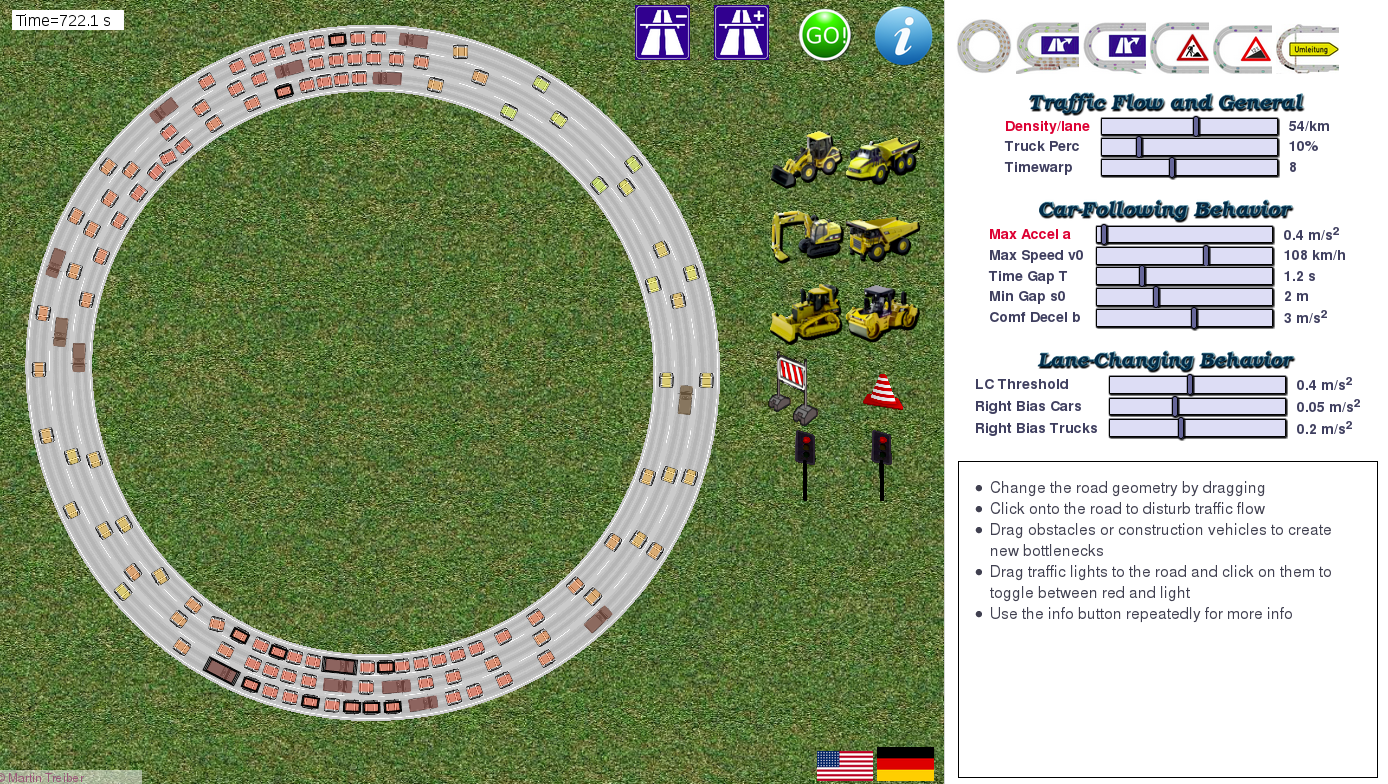
\includegraphics[width=70mm]{figs/screen_ringroad.png} &
  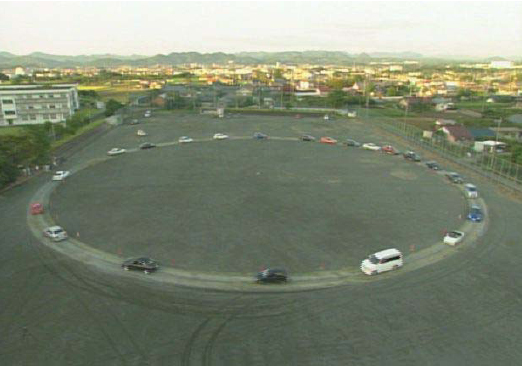
\includegraphics[width=60mm]{figs/nj265378fig2.jpg} 
\end{tabular}

 \caption{\label{fig:ringroadScenario}Left: Simulation screenshot for
   an increased density; right: a real-world experiment~\cite{Sugiyama-NJP08}.}

\end{figure}
%###################################################

As bottomline, we learn from this ring scenario the following:
 \begin{itemize}
\item Traffic waves always propagate \textit{against} the direction of
  the traffic flow at a velocity of about~\unit[15]{km/h} which does
  not depend on the system size, the initial or boundary conditions, the
  perturbations, or the traffic context (city, country road, freeway,
  change the free-flow speed for that). 
This is a sort of \textit{universal traffic
    flow constant}.  It is observed in real-world traffic worldwide (cf. right plot in Fig.~\ref{fig:ringroadScenario} from Ref.~\cite{Sugiyama-NJP08}).
\item 
The outflow of all types of moving
downstream fronts of congested traffic (per lane) is about the
same. This includes stop-and-go waves but also dissolving queues in
city traffic when the traffic light gets green. This so-called
\textit{dynamic capacity} is by typically \unit[10-20]{\%} lower than
the static capacity of the road. The resulting \textit{capacity drop}
is the reason why avoiding a traffic flow breakdown is crucial and
traffic jams resolve so slowly. 
\end{itemize}
%########################################################



\subsection{Open System Scenarios with Stationary Bottlenecks}
The simulator provides four scenarios with open boundaries and several
forms of infrastructure bottlenecks (Fig.~\ref{fig:openScenarios}):
On-ramp, off-ramp, roadworks (lane closing), and
an uphill section.


\begin{itemize}
\item
With the initial settings of the respective simulation, traffic breaks
down at or near the bottleneck region which, then, triggers upstream
propagating traffic waves.
\item 
Once the waves have formed, you can slow down the simulation speed
and click at an entering vehicle to observe how it encounters
seemingly \gquote{phantom} traffic waves. 
\item
As in the ring scenario, reduced traffic (controlled by the inflow
rather than the density) and a higher driver's responsiveness will
make the waves (but not necessarily the congestion) disappear.
\item 
Also \emph{off-ramps} may act as bottlenecks even though traffic
\emph{leaves} the road,  so, naively, one could think of an
\gquote{anti-bottleneck}.
\item Change the speed limit in the lane closing scenario and
  observe that traffic does not break down at the initial setting
  (limit 80 km/h) but for higher (and also lower!) speed
  limits. Notice the strong capacity drop in this case.
\item
Even locally changed driving characteristics, e.g., at curves or uphill
sections, may serve as a bottleneck. Reduce the maximum speed a truck
can drive at the uphill section and play with the truck overtaking
ban.
\item Before a breakdown has occurred, click on a vehicle in the
  bottleneck region to apply a disturbance. Notice how this vehicle
  triggers a breakdown although the driver may not even notice it!
\end{itemize}

%###################################################
\begin{figure}[!th]
\centering
\begin{tabular}{c}
  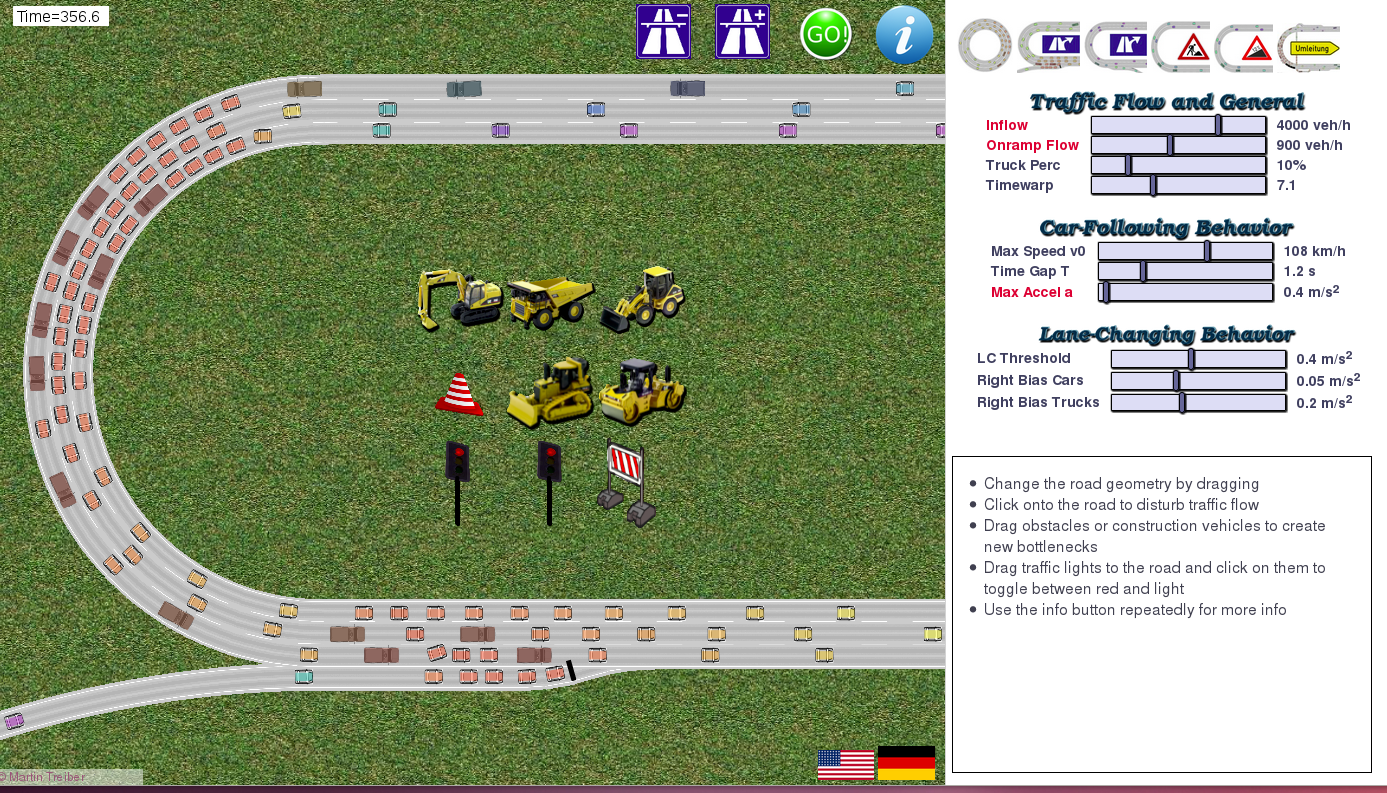
\includegraphics[width=90mm]{figs/screen_onramp.png} \\\\[1ex]
  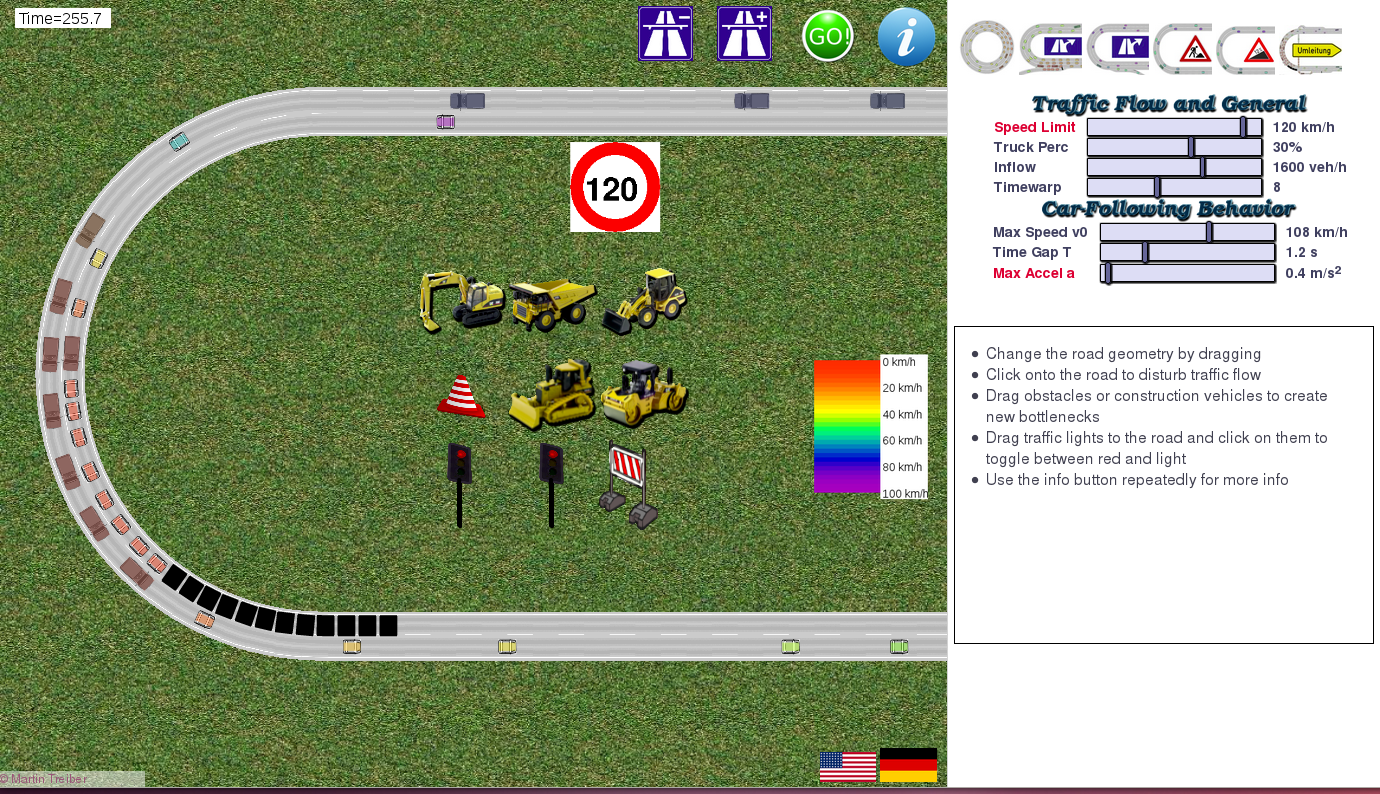
\includegraphics[width=90mm]{figs/screen_roadworks.png} \\\\[1ex]
  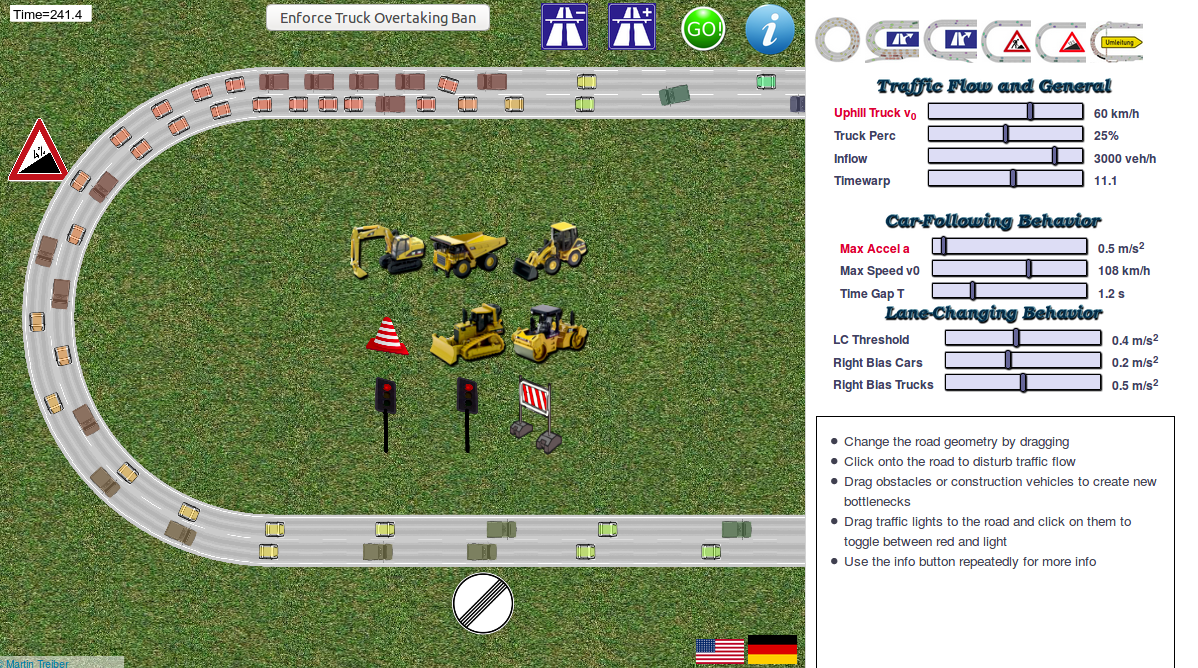
\includegraphics[width=90mm]{figs/screen_uphill.png}\\
\end{tabular}

 \caption{\label{fig:openScenarios}Screenshots of the open-system scenarios with different bottlenecks. The onramp represents a non-flow-conserving bottleneck. The flow-conserving bottlenecks differ in their strength: The lane closure is a strong inhomogeneity while the uphill grade is a mild one affecting only the trucks.}

\end{figure}
%###################################################

As bottomline, we learn from these scenarios the following:
\bi
\item In reality, phantom jams are not really \gquote{phantom} but they
have a cause and that cause is the bottleneck downstream: Because of
its invisibility (the bottleneck may be several kilometers downstream)
and the apparent causality (the driver encounters the effect before
the cause) the illusion of a phantom jam appears: There is always a
weakest ink.
\item The bottlenecks come in many forms. Their common and defining
  aspect is a local decrease of
the road capacity, i.e., its maximum throughput without causing
congestions.
\item Generally, we have \textit{three ingredients to make a jam}:
  High traffic demand, a bottleneck, and a local disturbance, e.g.,
  caused by a lane changing or by the user clicking on a vehicle.
\item Traffic managing measures such as speed limits try reduce the
  local disturbances and thereby prevent/delay a breakdown. One could
  say that \emph{slower is faster} or, 
  regarding ramp metering, \emph{less is more}. 
\ei


%########################################################
\subsection{Routing Game}\label{sec:routing}
In the final \gquote{deviation} scenario of the simulator, you can simulate
the effects of routing recommendations issued, e.g., by navigation
devices or variable message signs on the road. Play with the
\emph{deviation use} slider and notice that one can do too much of a
good thing: Instead of a mainroad jam behind the lane closing, traffic
on the deviation may break down. Since the deviation route has a much
lower capacity, a congestion on it will take much more time to
resolve.

Play the \gquote{routing game} and try to control traffic flow by the
\emph{deviation use} slider with the objective of bringing all
vehicles (there is only a fixed number) through the simulation in the
shortest time!

%###################################################
\begin{figure}[!th]
\centering
\begin{tabular}{c}
  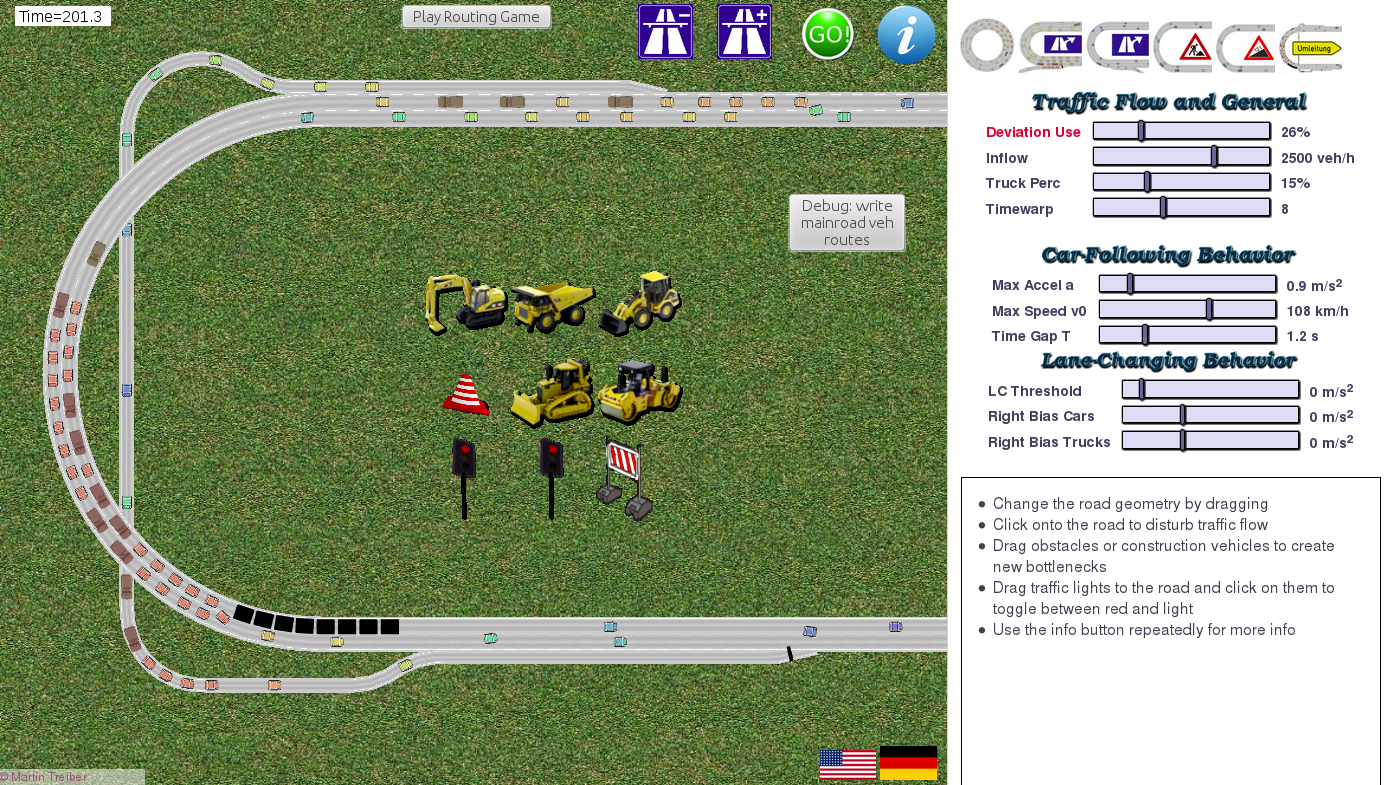
\includegraphics[width=90mm]{figs/screen_routing.png}
\end{tabular}
 \caption{\label{fig:routingScenario}Screenshot of the simulation scenario \gquote{Routing Game}.}
\end{figure}
%###################################################

\paragraph{Lessons learnt.}
Navigation and routing may be tricky since there is a delay between
the decision point (taking the main road or the deviation) and the
consequences (traffic jam on either road). Generally, a feedback
control with delays tends to be unstable. In our case, if you do not watch out
carefully, you will cause \emph{routing oscillations}.

%########################################################

\bibliographystyle{prsty} 
%\bibliography{database}

\begin{thebibliography}{1}

\bibitem{Opus}
M. Treiber, A. Hennecke, and D. Helbing, Physical Review E {\bf 62},  1805
  (2000).

\bibitem{TreiberKesting-Book}
M. Treiber and A. Kesting, {\em Traffic Flow Dynamics: Data, Models and
  Simulation} (Springer, Berlin, 2013).

\bibitem{MOBIL-TRR07}
A. Kesting, M. Treiber, and D. Helbing, Transportation Research Record {\bf
  1999},  86  (2007).

\bibitem{TreiberNumerics2015}
M. Treiber and V. Kanagaraj, Physica A: Statistical Mechanics and its
  Applications {\bf 419},  183   (2015).

\bibitem{Sugiyama-NJP08}
Y. Sugiyama {\it et~al.}, New Journal of Physics {\bf 10},  033001  (2008).

\end{thebibliography}

\end{document}



